\chapter{Oasis App}
\label{ch:App}
In this chapter we describe the Oasis App. The Oasis App is an application, which demonstrates some of the utilities the Oasis Lib offers. First the design of the Oasis App is described in Section \vref{sec:AppDesign}. After that the implementation of the Oasis Lib in the Oasis App is described in Section \vref{sec:AppImp}.

\section{Design}
\label{sec:AppDesign}
The idea behind the Oasis App is that we want to make a tool, for the guardians, to manage the profile data, by giving them CRUD (Create, Read, Update, and Delete) options.

The application design should be revolving around the database structure with the key functionality being profile handling.
The application design has been divided into two parts; the home screen of the application and an overview screen showing relevant data.

Paper prototypes of the GUI has been created and evalutated.
Several prototypes have been made and the chosen prototype for the application can be seen in Figure \vref{fig:homeScreenProto} and Figure \vref{fig:overviewScreenProto}.

\begin{figure}[H]
	\centering
		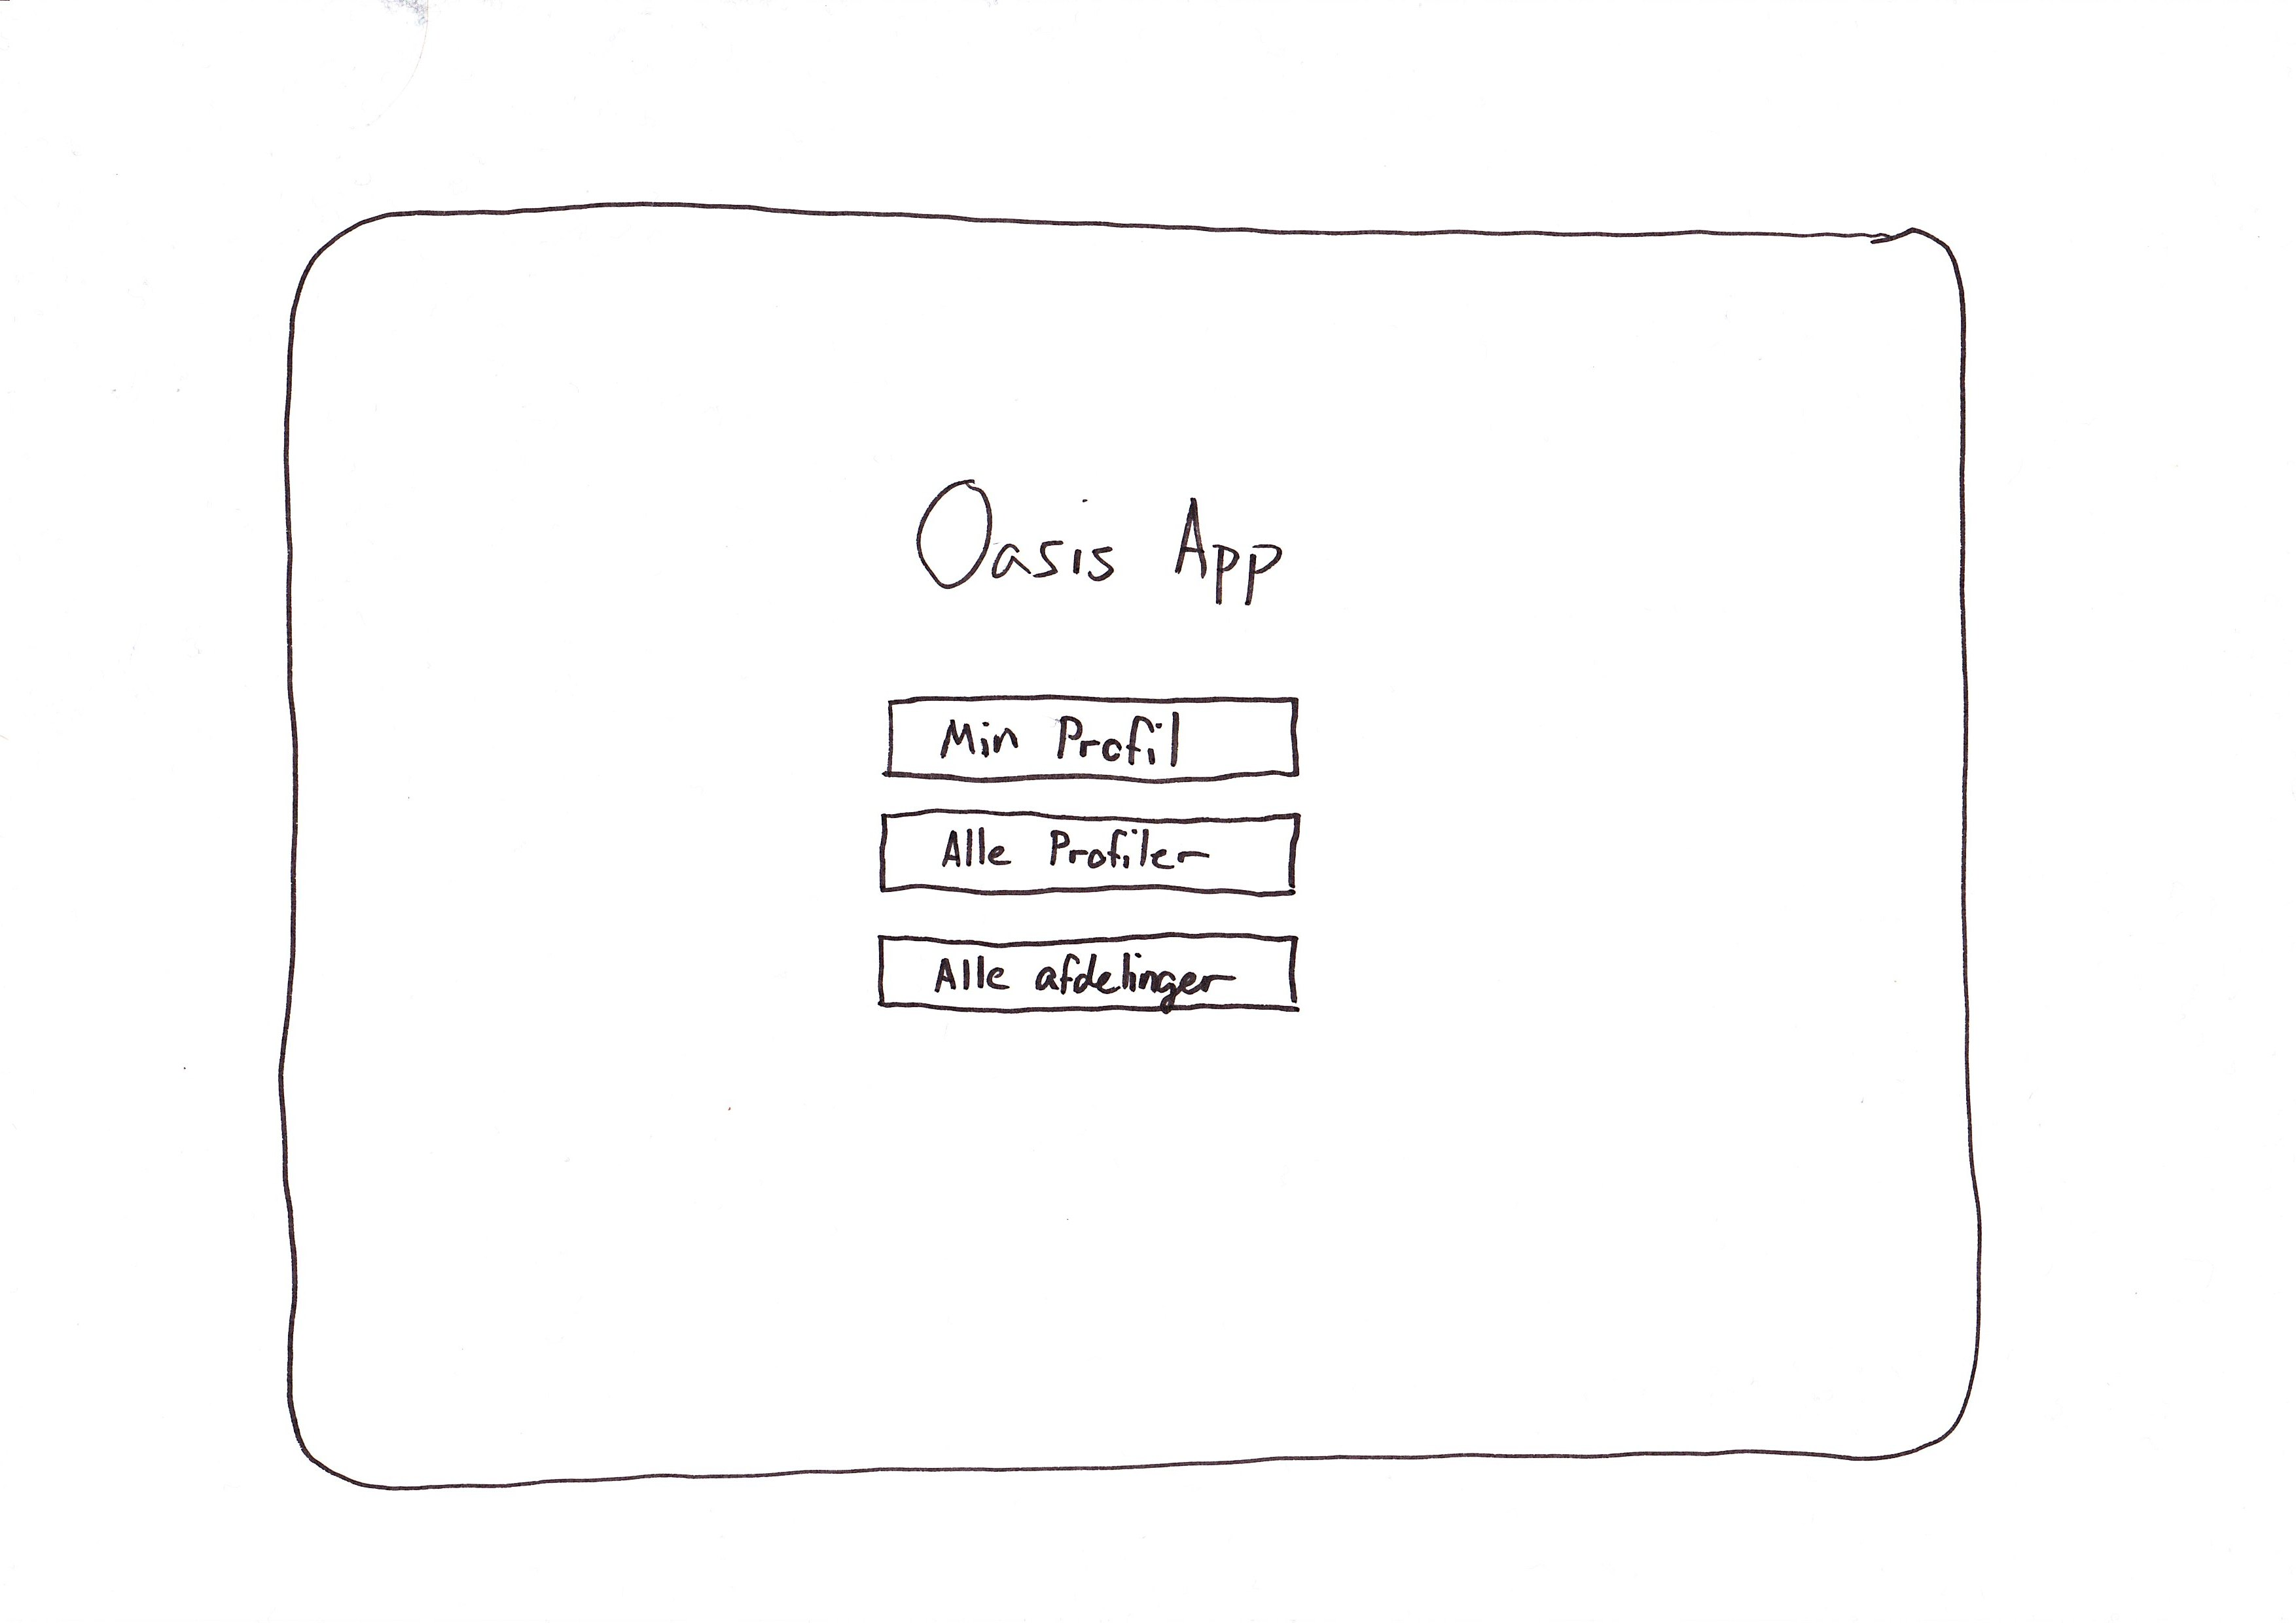
\includegraphics[width=0.9\textwidth]{Images/homeScreenPrototype}
	\caption{The prototype for the home screen.}
	\label{fig:homeScreenProto}
\end{figure}

\begin{figure}[H]
	\centering
		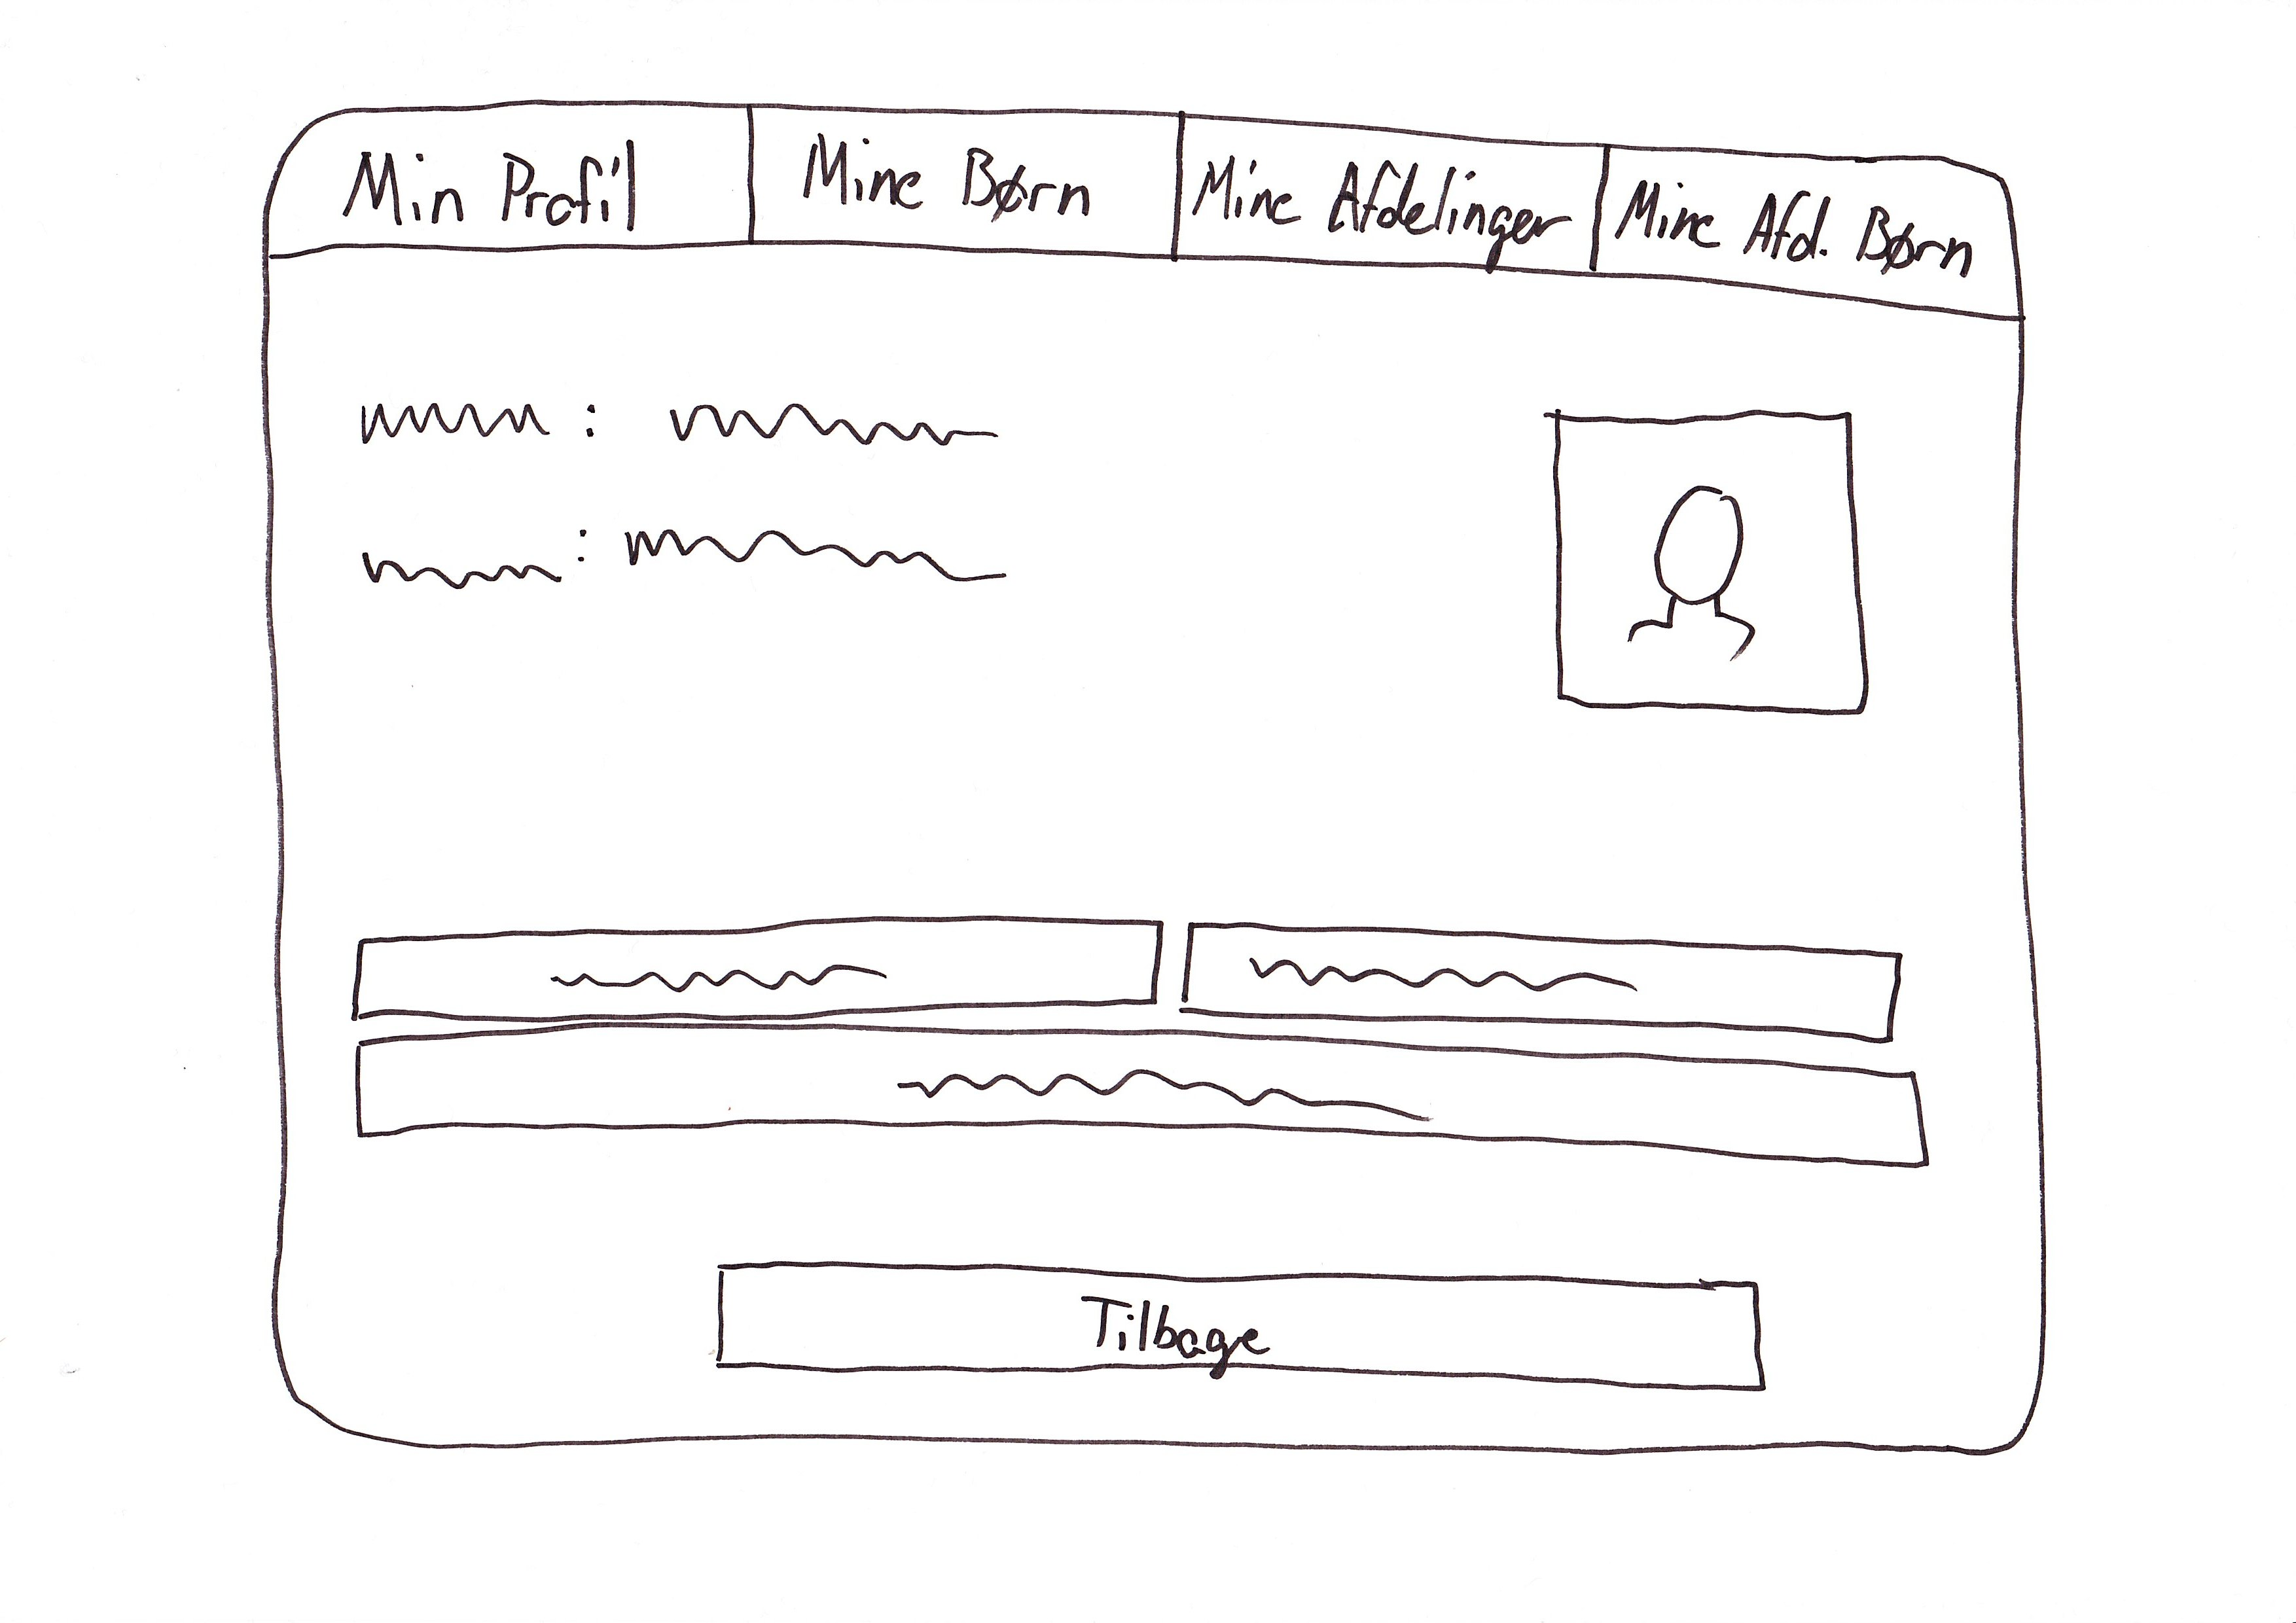
\includegraphics[width=0.9\textwidth]{Images/overviewScreenPrototype}
	\caption{The prototype for the overview screen.}
	\label{fig:overviewScreenProto}
\end{figure}

The final prototypes have been implemented as the GUI in the Oasis App.

\section{Implementation}
\label{sec:AppImp}
The Oasis App is split into two activities; \texttt{MainActivity} and \texttt{FragParentTab}.

\subsection{MainActivity}
The \texttt{MainActivity} is the activity that starts at application startup. It uses the main.xml as its layout file, which is a layout file containing three buttons, which can be seen on Figure \vref{fig:homeScreen}. 

\begin{figure}[H]
	\centering
		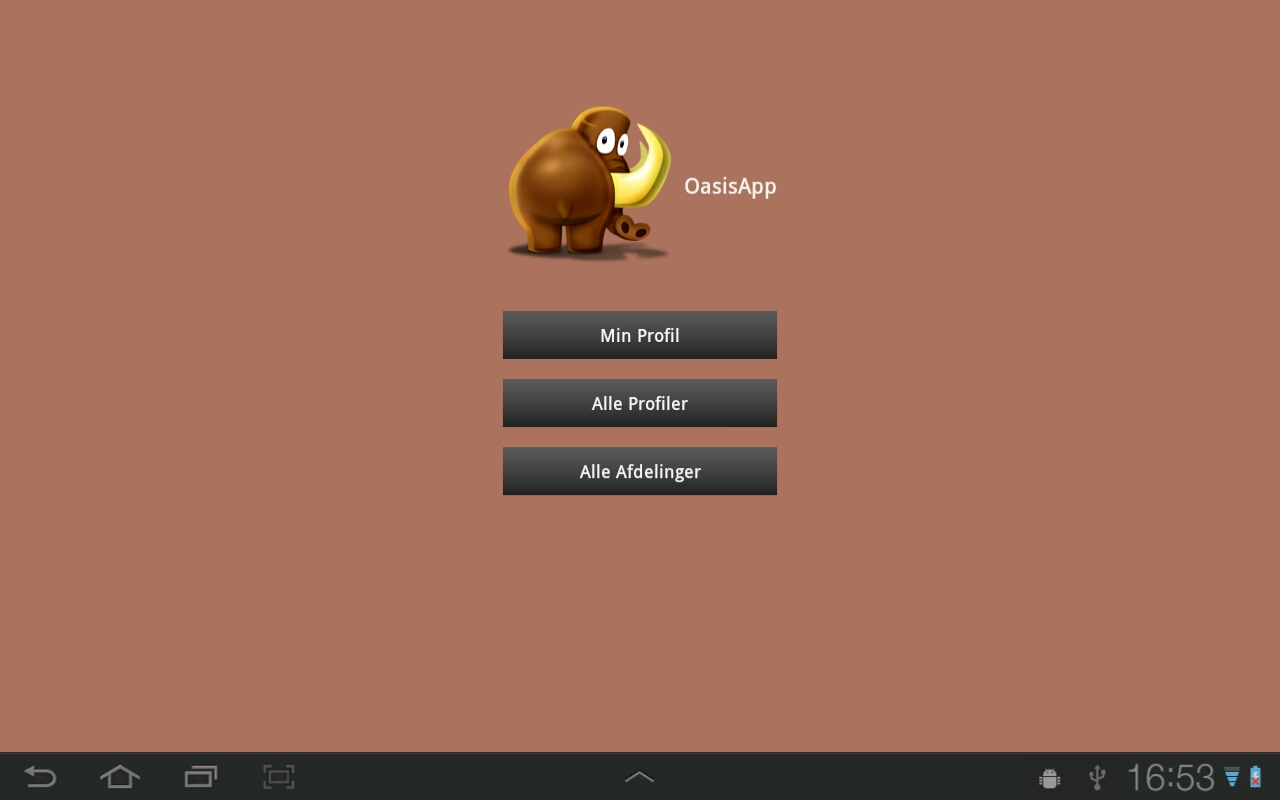
\includegraphics[width=\textwidth]{Images/homeScreen}
	\caption{An image of the \texttt{MainActivity} layout.}
	\label{fig:homeScreen}
\end{figure}

A code snippet of the MainActivity's code can be seen in Listing \vref{lst:mainactivity}.

\begin{Java}{The MainActivity class}{lst:mainactivity}
.
.
.
public class MainActivity extends Activity implements OnClickListener {

	private Button bMyProfile, bAllProfiles, bAllDepartments, bAddDummyData;
	private Intent direct;
	private long guardianId;
	public Helper helper;
	public static Profile guardian;
	public static Profile child;
	public static int color;

	@Override
	public void onCreate(Bundle savedInstanceState){
		super.onCreate(savedInstanceState);

		.
		.
		.

		helper = new Helper(this);

		Bundle extras = getIntent().getExtras();
		if (extras != null) {        	   
			guardianId = extras.getLong("currentGuardianID");
			color = extras.getInt("appBackgroundColor");
			guardian = helper.profilesHelper.getProfileById(guardianId);
		}

		setContentView(R.layout.main);
		
		initializeViews();
	}

	private void initializeViews() {
		findViewById(R.id.UpperLayout).setBackgroundColor(color);
		
		bMyProfile = (Button) findViewById(R.id.bMyProfile);
		bMyProfile.setOnClickListener(this);
		bAllProfiles = (Button) findViewById(R.id.bAllProfiles);
		bAllProfiles.setOnClickListener(this);
		bAllDepartments = (Button) findViewById(R.id.bAllDepartments);
		bAllDepartments.setOnClickListener(this);
		bAddDummyData = (Button) findViewById(R.id.bAddDummyData);
		if (guardian == null) {
			bAddDummyData.setOnClickListener(this);
		} else {
			bAddDummyData.setVisibility(View.GONE);
		}
	}

	@Override
	public void onClick(View v) {
		direct = new Intent(this, FragParentTab.class);

		switch (v.getId()) {
		case R.id.bMyProfile:
			if (guardian != null) {
				direct.putExtra("tabView", FragParentTab.TABPROFILE);
				startActivity(direct);
			} else {
				Toast.makeText(this, R.string.noprofile, Toast.LENGTH_SHORT).show();
			}
			break;
		case R.id.bAllProfiles:
			direct.putExtra("tabView", FragParentTab.TABALLPROFILES);
			startActivity(direct);
			break;
		case R.id.bAllDepartments:
			direct.putExtra("tabView", FragParentTab.TABALLDEPARTMENTS);
			startActivity(direct);
			break;
		.
		.
		.
		}
	}
}
\end{Java}

As the activity starts it gets the information of which guardian who is currently logged in to the GIRAF system and what background color the Oasis App is currently set to by the Launcher.
When one of the buttons is clicked, the \texttt{MainActivity} will start the \texttt{FragParentTab} activity and put the corresponding integer in the intent's extra data.

\subsection{FragParentTab}
The FragParentTab is the activity, which is started by the \texttt{MainActivity} activity.
The activity has the responsibillity of managing what view to show, by using fragments.
We chose fragments because we wanted a tab layout.
An example of the tab layout view can be seen in Figure \vref{fig:overviewScreen}.

\begin{figure}[H]
	\centering
		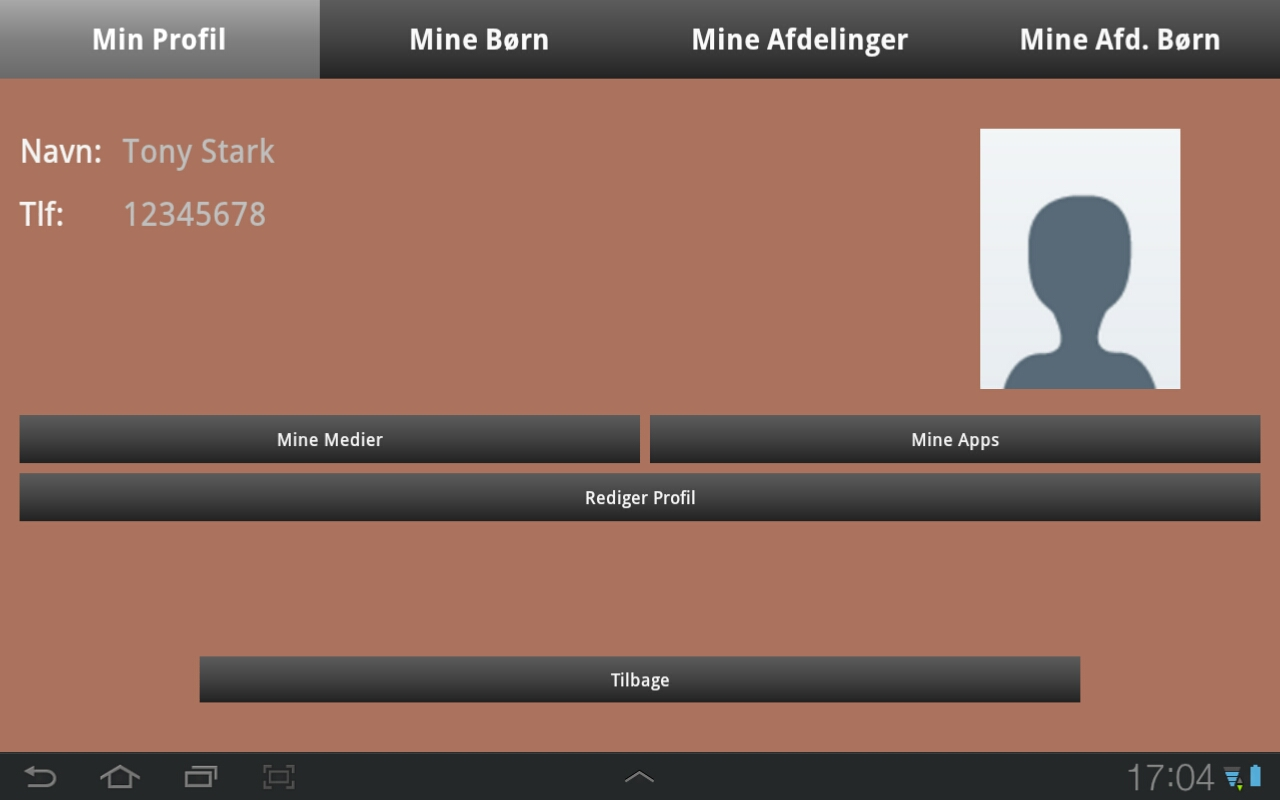
\includegraphics[width=\textwidth]{Images/overviewScreen}
	\caption{An image of the \texttt{FragParentTab} layout.}
	\label{fig:overviewScreen}
\end{figure}

The FragParentTab activity can be seen in Listing \vref{lst:fragparenttab}.

\begin{Java}{The FragParentTab class}{lst:fragparenttab}
.
.
.
public class FragParentTab extends Activity {

	private int tabView;
	public final static int TABPROFILE = 0;
	public final static int TABAPP = 1;
	public final static int TABMEDIA = 2;
	public final static int TABALLPROFILES = 3;
	public final static int TABALLDEPARTMENTS = 4;
	public final static int TABCHILD = 5;
	public final static int TABCHILDAPP = 6;
	public final static int TABCHILDMEDIA = 7;
	static FragmentManager t;

	@Override
	protected void onCreate(Bundle savedInstanceState) {
		super.onCreate(savedInstanceState);

		.
		.
		.

		Bundle extras = getIntent().getExtras();
		if (extras != null) {
			tabView = extras.getInt("tabView");
		} else {
			tabView = -1;
		}

		setContentView(R.layout.fragments_view);
		
		findViewById(R.id.fragUpperLayout).setBackgroundColor(MainActivity.color);

		t = getFragmentManager();

		switch(tabView) {
		case TABPROFILE:
			t.beginTransaction().add(R.id.fDetails, new TabManagerProfile()).commit();
			break;
		case TABALLPROFILES:
			t.beginTransaction().add(R.id.fDetails, new TabManagerAllProfiles()).commit();
			break;
		case TABALLDEPARTMENTS:
			t.beginTransaction().add(R.id.fDetails, new TabManagerAllDepartments()).commit();
			break;
		case TABCHILD:
			t.beginTransaction().add(R.id.fDetails, new TabManagerChild()).commit();
		}
	}

	public static void switchTab(int tabViewId) {

		switch(tabViewId) {
		case TABPROFILE:
			t.beginTransaction().replace(R.id.fDetails, new TabManagerProfile()).commit();
			break;
		case TABMEDIA:
			t.beginTransaction().replace(R.id.fDetails, new TabManagerMedia()).commit();
			break;
		case TABAPP:
			t.beginTransaction().replace(R.id.fDetails, new TabManagerApp()).commit();
			break;
		case TABCHILD:
			t.beginTransaction().replace(R.id.fDetails, new TabManagerChild()).commit();
			break;
		case TABCHILDMEDIA:
			t.beginTransaction().replace(R.id.fDetails, new TabManagerChildMedia()).commit();
			break;
		case TABCHILDAPP:
			t.beginTransaction().replace(R.id.fDetails, new TabManagerChildApp()).commit();
			break;
		}
	}
	
	@Override
	protected void onResume() {
		super.onResume();
		t = getFragmentManager();
	}
}
\end{Java}

The activity controls which fragment it must show and this is done in two ways.
The first way is when the activity is created, it decides which fragment to show, by using the integer it gets from the \texttt{MainActivity}.
This integer represents a fragment class of every tab layout view.
This fragment is then added to the fragment stack.

The other way is when a fragment wants to replace itself with another fragment.
Here the fragment calls the switchTab method, in the \texttt{FragParentTab} activity, with the replacing view integer as a parameter.

\subsection{Utilizing the Oasis Lib}
Before utilizing the methods within the Oasis Lib, the developer must include the library.
It is also necassary to instantiate a helper object before it can be used.
When instantiating the object it is necassary to input the current activity's context as a parameter.
This is needed to give the Oasis Lib the information about where it is called from.
An example of how to instantiate the helper object, can be seen in Listing \vref{lst:initHelper}.

\begin{Java}{Example of Instantiating a helper object.}{lst:initHelper}
Helper helper = new Helper(getActivity().getApplicationContext());
\end{Java}

After the instantiation it is possible to call all the methods within the Oasis Lib.
An example of calling a method can be seen in Listing \vref{lst:callLib}.

\begin{Java}{Call method from the Oasis Lib.}{lst:callLib}
guardian = helper.profilesHelper.getProfileById(guardianId);
\end{Java}